\documentclass[11pt]{article}
\usepackage[utf8]{inputenc}
\usepackage{helvet}
\renewcommand{\familydefault}{\sfdefault}
\usepackage[margin = 0.75in]{geometry}
\usepackage{graphicx}
\usepackage{wrapfig}
\usepackage{pdfpages}
\usepackage{svg}
\usepackage{amsmath}
\usepackage{hyperref}
\setlength{\parskip}{1em}
\usepackage{wrapfig}
\usepackage[font=small,labelfont=bf]{caption}
\usepackage{titlesec}

\usepackage[citestyle = authoryear]{biblatex}
\addbibresource{sources.bib}

\titlespacing{\section}{0pt}{\parskip}{-\parskip}
\titlespacing{\subsection}{0pt}{\parskip}{-\parskip}
\titlespacing{\subsubsection}{0pt}{\parskip}{-\parskip}



\title{MECHENG 706 Project 1}
\author{Calvin Lee, Freeman Porten, Jake Olliff and Lachlan Barnes}
\date{April 2020}

\begin{document}

\maketitle

\section{Summary}
\begin{figure}[htbp]
    \centering
    \includegraphics[width=10cm]{3rdAngleView.jpg}
    \caption{}
    \label{fig:3rdAngleRobot}
\end{figure}
\section{Sensing System - By Jake Olliff}

\section{Open-Loop Control - By Calvin Lee}

\newpage
\section{Closed-Loop Control - By Freeman Porten}

\par To fulfil the precise wall following requirement of the project a closed loop control system was required to keep the distance from the wall a constant 15cm and keep the robot aligned parallel with the wall. The control system that was chosen was Proportional Integral Derivative control (PID). A PID system was chosen as it has a good balance between precision, stability and complexity. Another advantage of PID control is that it does not require the calculation of the robots transfer function, instead the open loop response of the robot can be used for obtaining initial gains.

\subsection{Inverse Kinematic Equations} \label{sec:KinematicEquations}

\par Before designing the control system, it was first necessary to obtain a set of equations for the inverse kinematics of the robot. Equations \ref{eq:InverseKinematics:1}, \ref{eq:InverseKinematics:2}, \ref{eq:InverseKinematics:3} and \ref{eq:InverseKinematics:4} give the required speed of the left front ($\omega_{1}$) , left rear ($\omega_{2}$), right front($\omega_{3}$) and right rear ($\omega_{4}$) wheels for a desired rotation speed ($\omega_{z}$), forwards speed ($V_{x}$) and strafing speed ($V_{y}$) of the robot, see figure \ref{fig:WallFollow} for coordinate system definition of robot. These equations were obtained from the lecture slides and then tested on the robot to ensure validity.
\begin{align}
    \omega_{1} &= V_{x} + V_{y} - (l_{x} + l_{y})\omega_{z}\label{eq:InverseKinematics:1}\\ 
    \omega_{2} &= V_{x} - V_{y} - (l_{x} + l_{y})\omega_{z}\label{eq:InverseKinematics:2}\\ 
    \omega_{3} &= V_{x} - V_{y} + (l_{x} + l_{y})\omega_{z}\label{eq:InverseKinematics:3}\\ 
    \omega_{4} &= V_{x} + V_{y} + (l_{x} + l_{y})\omega_{z} \label{eq:InverseKinematics:4}
\end{align}
\subsection{Position Tracking}
\begin{wrapfigure}{r}{0.4\textwidth}
    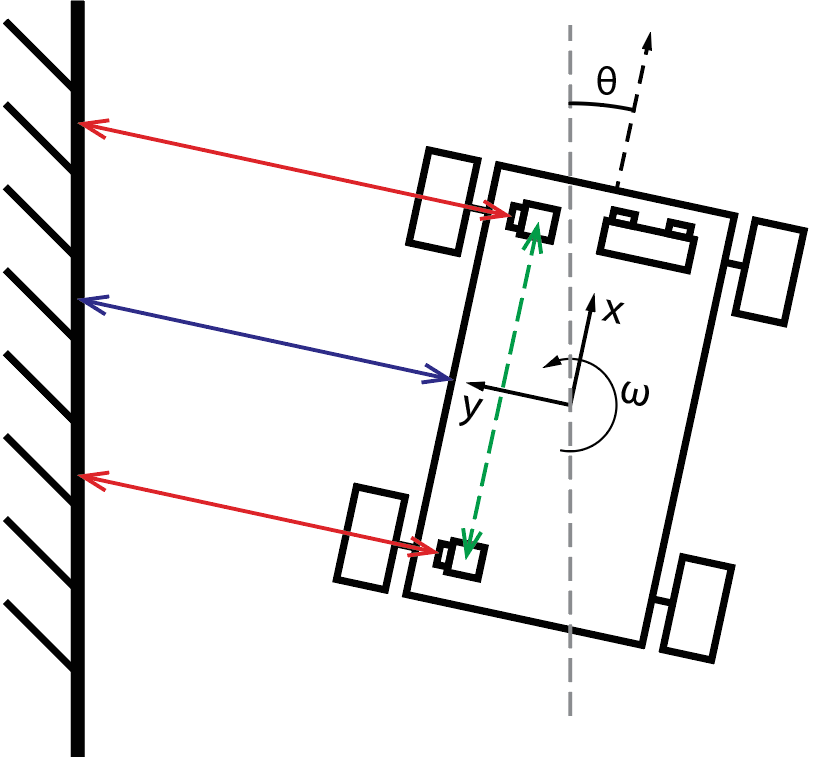
\includegraphics[width=0.35\textwidth]{WallFollow.PNG}
    \caption{Diagram of relevant distances for wall following, red arrows are the IR sensor distances $IR_{r}$ and  $IR_{f}$, the blue arrow is the average distance from the wall, the green dashed arrow is $l_{IR}$ and $\theta$ is the angle of the robot relative to the wall.}
    \label{fig:WallFollow}
\end{wrapfigure}

\par To control the robot we first need to know where the robot is relative to the wall it is trying to follow. The distance from the wall is calculated by taking the average of the distances read by the front and rear IR sensors $IR_{r}$ and  $IR_{f}$ respectively, see the blue arrow in figure \ref{fig:WallFollow}. Finding the distance to the wall in front of the robot is similarly simple, this is done using the Sonar Sensor mounted on the front of the robot.

The angle of the robot relative to the wall can be calculated with $\tan(\frac{IR_{r} - IR_{f}}{2l_{x}})$ Where $l_{IR}$ is the distance between IR sensors on the x axis, see green dashed arrow on figure \ref{fig:WallFollow}. Use of trig functions can lead to non-linearity issues and infinite values. We only need our angle to be accurate when the angle is small as when the angle is large we will have actuator saturation in the wheel motors anyway. That means that using the small angle approximation $tan(\theta) = \theta$ the complexity of the calculations can be reduced while still maintaining sufficient accuracy. Thus 

\subsection{PID Control}

\subsection{Controller Design}
\par Once the robot has an idea of where it is relative to the wall a control system can be implemented to drive it to some reference values. This was done with the use of 3 PID controllers, figure \ref{fig:PIDControl} shows a the control system block diagram that was implemented in our design. The 3 PID controllers control the 3 input variables of the inverse kinematic equations described in section \ref{sec:KinematicEquations}. The controllers will drive the error between measured position relative to the wall and the desired reference position to zero. When following a wall the references are set to 0mm, 150mm and 0rad for the X Ref, Y Ref and $\omega$ Ref respectively. The PID controllers turn the position errors into the three velocity inputs of the inverse kinematic equations as can be seen in figure \ref{fig:PIDControl}.

\begin{figure}[htbp]
    \centering
    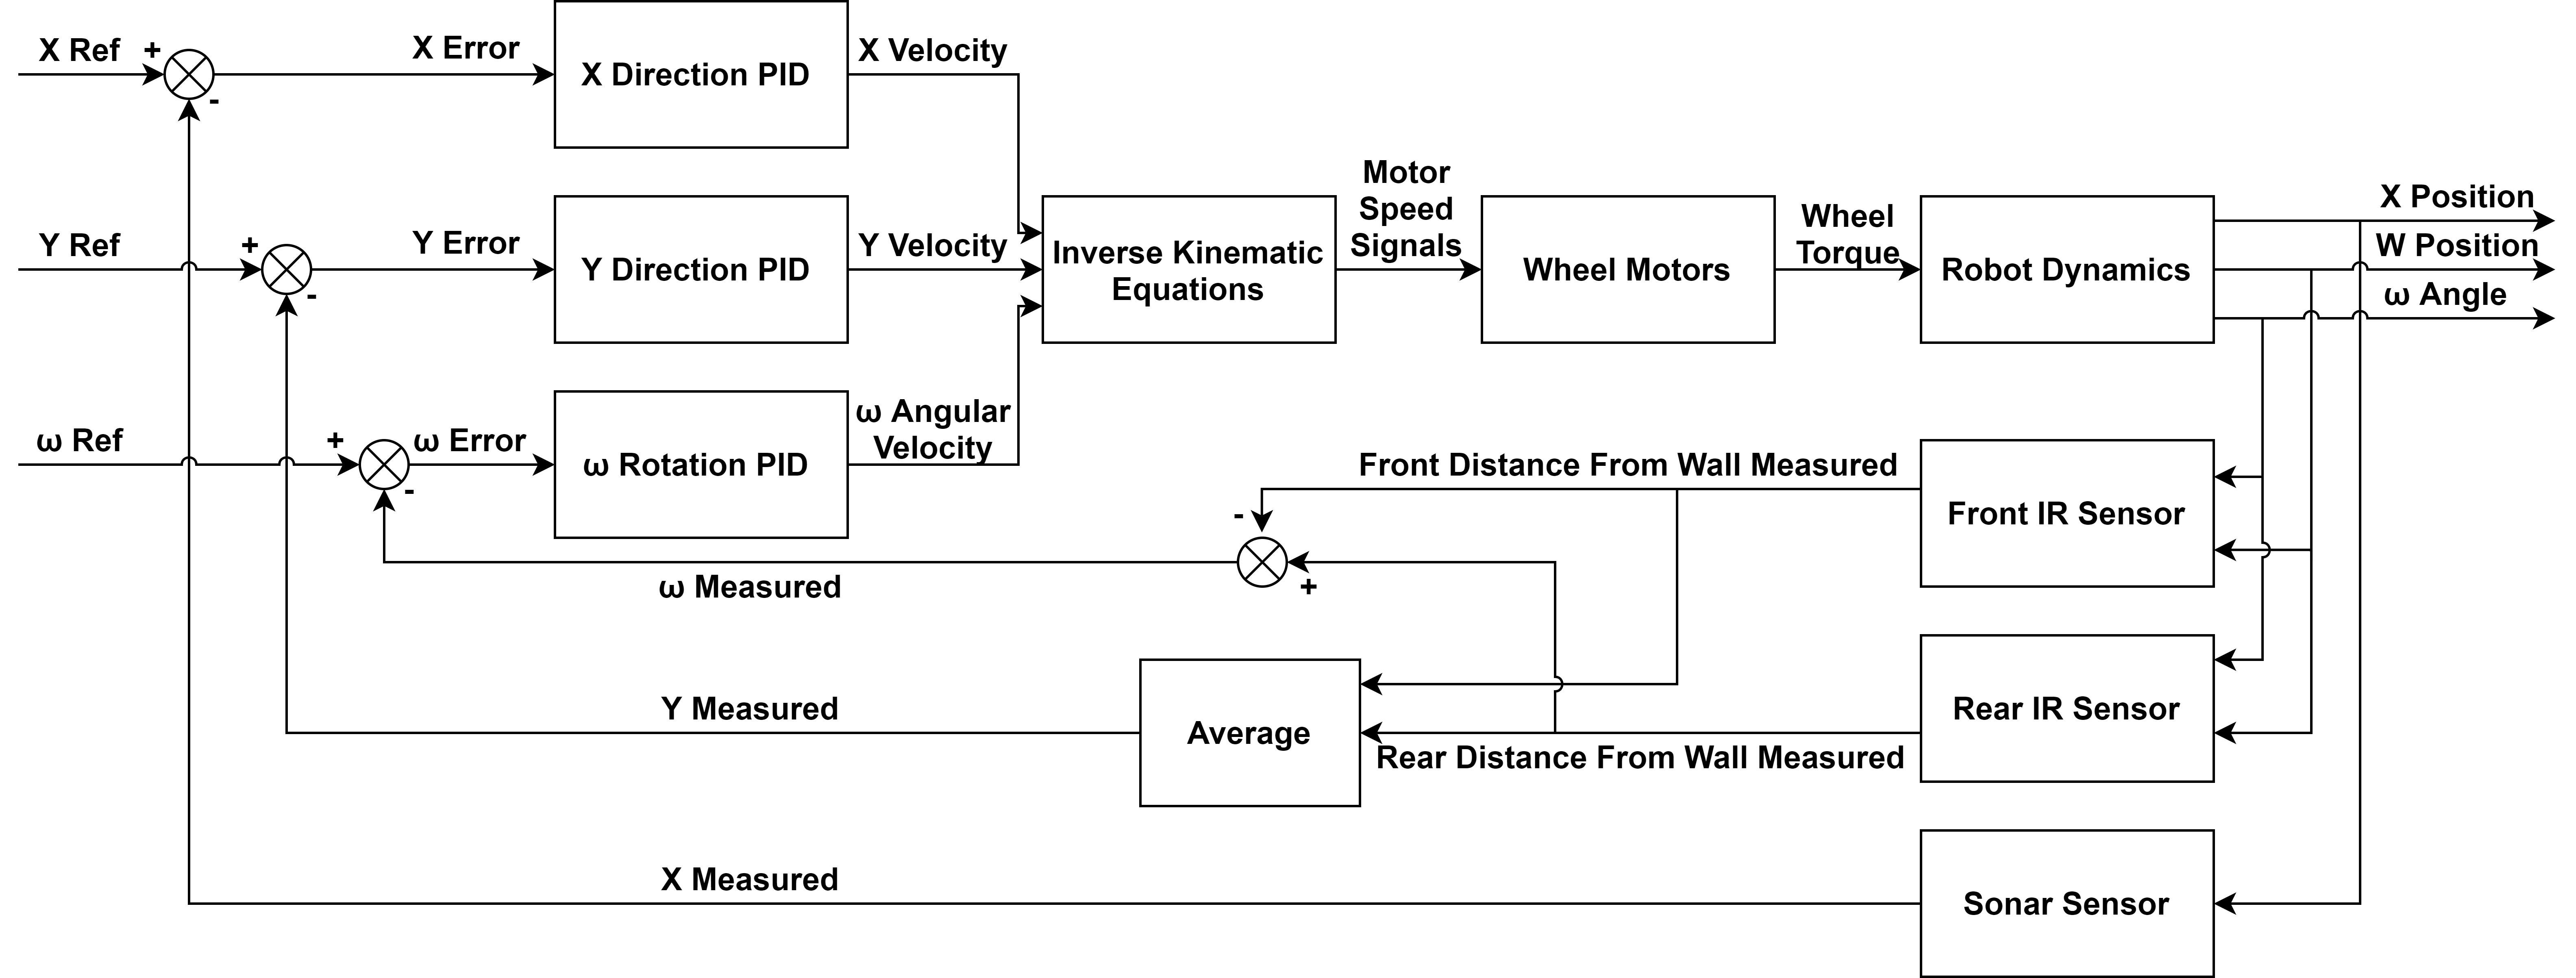
\includegraphics[width=0.9\textwidth]{ControlDiagram.png}
    \caption{Control System Block Diagram for Closed-Loop Wall Following}
    \label{fig:PIDControl}
\end{figure}

\par The arduino PID library written by Brett Beauregard was used as the basis for the PID controllers (\cite{beauregardPID}). This PID library contained some useful additional features that solve some of the issues with PID control. One of the main issues with PID control is actuator saturation causing integrator windup. When the motors reach their maximum speed, the integral term of the controller will continue summing in an attempt to raise the motor above the maximum speed. This will cause the the robot to have a large overshoot response. To eliminate this issue we can tell the controller to stop summing the integrator when the motors are saturated. In addition to this the code will also prevent the proportional and derivative terms from attempting to raise the motors above their maximum speed. The library also allows to switch to manual control of the motors and back without causing the motors speed to spike due to the integral and derivative terms. This is useful when we want to switch to closed-loop control after using open-loop control to turn a corner. When leaving manual mode the integrator term was reset and the previous input value was set to be equal to the current input value so that the derivative term sees zero change in input.

\subsection{Controller Tuning}
To be completed

\newpage
\section{Software-Hardware Integration - By Lachlan Barnes}

\section{Conclusion}
\printbibliography
\end{document}
